\section{Results and Discussion} \label{sec:results}

\subsection{Runtime Comparison}

In direct comparison between the naive and the shortcut-enabled trie building implementations, we found substantial improvements in execution time under by the latter.
Figure~\ref{fig:comparison} compares execution time for both approaches for problem sizes ranging up to 10,000 genomes.
Over this window, the naive algorithm's runtime appears to grow at a superlinear pace, increase up to 15 minutes for the largest surveyed problem size.
In contrast, runtime for the shortcut-enabled approach at this scale is approximately 3 seconds --- a 300-fold difference in performance.

\begin{center}
\begin{figure}[h]
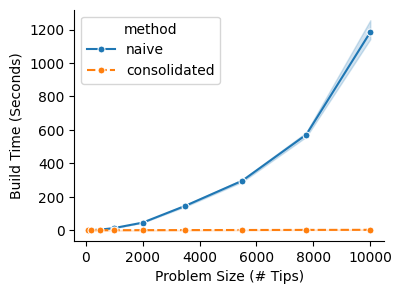
\includegraphics[width=\linewidth]{img/time_by_tips.png}
\caption{
\textbf{Microbenchmark comparison of naive trie and shortcut table algorithms.}
\small
Naive approach appears to exhibit superlinear scaling.
Shaded bands are 95\% confidence intervals, NUM\_TODO samples per observation.
}
\label{fig:comparison}
\end{figure}
\end{center}

Although Python code was used for both algorithms in this trial to ensure apples-to-apples comparability, implementations did differ in the underlying data structure used to store trie data.
The shortcut-enabled implementation used a contiguous edge-list table to store trie data, while the naive implementation used a node-and-pointer approach.
Typically, table-based approaches are faster in practice due to cache locality effects and reduced memory allocation calls.
However, both data structures provide equivalent time complexities for all relevant initialization and lookup operations.
Thus, the notable difference in scaling properties between the shortcut-enabled and naive benchmarks is indicative of meaningful differences in the underlying algorithms, beyond effects attributable to data structure implementations.

\subsection{Microbenchmark: Empirical Scaling Analysis}

\begin{figure*}[t]
  \centering
  \begin{minipage}{0.33\textwidth}
    \centering
    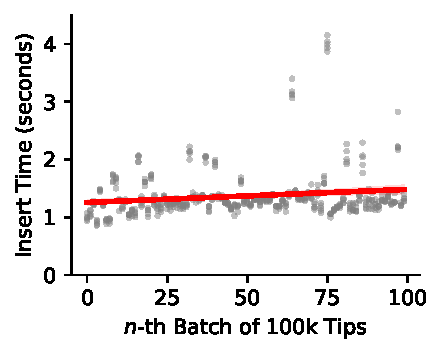
\includegraphics[height=4.3cm]{img/series-purifying.pdf}
    \vspace{-0.5em}
    \subcaption{Purifying Regime}
    \label{fig:scaling:purifying}
  \end{minipage}%
  \begin{minipage}{0.33\textwidth}
    \centering
    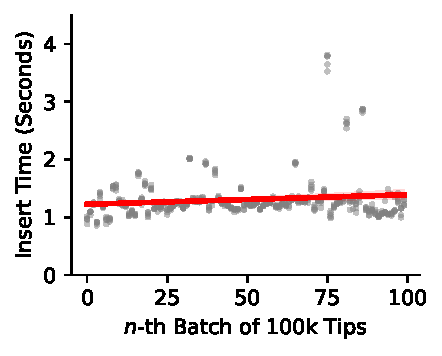
\includegraphics[height=4.3cm,trim={0.7cm 0 0 0},clip]{img/series-adaptive.pdf}
    \vspace{-0.5em}
    \subcaption{Adaptive Regime}
    \label{fig:scaling:adaptive}
  \end{minipage}%
  \begin{minipage}{0.33\textwidth}
    \caption{%
    \textbf{Empirical performance scaling of shortcut table algorithm in microbenchmark trials.} \small
    Panels \ref{fig:scaling:purifying} and \ref{fig:scaling:adaptive} differ in simulation data source of sampled genomes, with the former exhibiting higher phylogenetic richness. Data collected as batches are added in a 10 million tip reconstruction, sampled 5 times per panel. \vspace{2.5em}
}
    \label{fig:scaling}
  \end{minipage}
  \vspace{-1.5em}
\end{figure*}


Having seen a substantial speedup in comparing the shortcut-enabled algorithm to the naive trie-building approach, we next sought to assess the scaling properties of the shortcut-enabled approach in isolation.
To better reflect real-world conditions, we used the main C++ implementation of the trie-building algorithm for these trials.

Figure~\ref{fig:scaling} depicts the relationship between the tree size as 100 thousand tip batches are added and the time taken to insert each batch, over 5 samples of a 10 million tip reconstruction.
Fitting a simple linear regression model to this data, we found that, with a significance of $\alpha = 0.05$, that we should reject the null hypothesis of a constant slope, and infer that as tree sizes increase, the time taken to add tips increases as well.

Analyzing the graph, we see that these results seem to be a result of outliers within the data, most likely due to expensive consolidation steps. A more fine-grained analysis (with batches of 5000) on average-case data (filtering out values above the 95th percentile) shows that past a certain point, insertion times do not increase (see supplemental \citep{supplemental} for more information).

However, these outliers may be amortized away in practice -- after running the reconstruction on both adaptive and purifying regimes, we see approximately linear scaling in the time taken to reconstruct a tree from a given number of tips (see Figure~\ref{fig:asymptotic} in the supplemental material \citep{supplemental}).

\subsection{Macrobenchmark: One Billion-Tips}

\begin{figure}

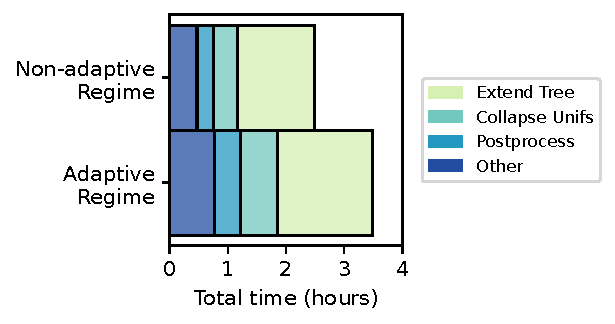
\includegraphics[width=3in]{binder/binder-2025_03_13_preliminary_billion_tip_reconstruction_graphing.ipynb/binder/teeplots/viz=plot-billion-tip-reconstruction-stack+ext=.pdf}

\caption{\textbf{Billion-tip reconstruction times.} TODO.}
\label{fig:billion-tip-time}
\end{figure}


Given the promising results of microbenchmark trials, particularly the favorable empirical scaling result, we next sought to assess the performance of our approach on an extremely large problem size.

For this purpose, we conducted trial reconstruction benchmarks comprising the full corpus of 1 billion agent genomes extracted from our trial Wafer-Scale Engine experiments.
As a point of comparison, the largest reconstructions performed using the previous approach comprised only 10,000 tips \citep{moreno2024trackable}.

% log files:
% https://osf.io/s3rzj and https://osf.io/gj52m
Benchmarked operations included the full reconstruction operation pipeline shown in Figure \ref{fig:hstratschematic}.
Input data comprised a Parquet format file storing raw agent genomes in a hexidecimal string representation.
The population file size was 34 GB for and 35 GB for the sample adaptive- and purifying-selection regimes, respectively.
The output data comprised the reconstructed phylogeny in an edge-list format closely resembling the ALIFE data standard.
Several pieces of metadata (e.g., agent position and extraction batch) were forwarded to the output data.
For the adaptive-selection regime, the output file size was 54 GB, and for the purifying-selection regime, the output file size was 55 GB.

% log files:
% https://osf.io/s3rzj and https://osf.io/gj52m
Given the large problem-size scale tested, macrobenchmark trials were carried out on a compute cluster node, rather than a desktop PC, as was used for microbenchmark experiments.
Figure \ref{fig:billion-tip-time} profiles net runtime and its breakdown in our case study reconstruction trials.
Reconstruction time was 2h:30m for the adaptive-regime data set.
As expected, given the associated richer phylogenetic history, reconstruction was more intensive for the purifying-regime data set, clocking in at 3h:29m.
These figures correspond to a net throughput of 6.67 and 4.78 million tips per minute, respectively.
Peak memory use for the adaptive and purifying selection regimes was 1.2 TB and 1.1 TB.

\subsection{Validation: Comparison to Ground Truth}

Finally, we conducted experiments to validate the quality of phylogenies produced by our algorithm.

We began by testing the accuracy of the reconstruction on ground-truth phylogenies.
For these trials, we conducted experiments using a neutral evolution model on a single CPU, where we were able to directly record the underlying phylogeny history. See the supplemental material for an example comparison between a ground-truth tree and estimated reconstruction \citep{supplemental}.

To assess reconstruction error, we used the triplet distance metric to compare corresponding ground-truth and estimated phylogenies.
This metric can be interpreted as the fraction of sampled three-node sets for which both trees report the same two nodes as more closely related.

%TODO can we also report SD of error (this will give a sense for distribution of error)
%MAYBE if time permits, it would be ideal to have a second row in this table where we have error measures from the naive algorithm
\begin{table}[h]
\vspace{-0.8em}
\centering
\begin{tabular}{r|c|c|c|c}
Surface Size & 8 & 16 & 32 & 64  \\
\hline 
Mean Error & 0.373 & 0.191 & 0.095 & 0.021 \\
Standard Deviation & 0.240 & 0.156 & 0.082 & 0.018 \vspace{-1.5ex} 
\end{tabular}
\caption{\textbf{Accuracy of shortcut table algorithm on simulated data.}
\small Mean error is defined as the average triplet distance between reconstructed and ground truth phylogenies over 20 random simulations of evolution, with each organism having a variable surface size. A steady retention policy was used.
}
\label{table:validation}

% 8: [0.49751863909599, 0.16413449038322647, 0.17574884165379615, 0.17641529350326116, 0.4970519672440805, 0.3426438071534128, 0.7352663918487983, 0.23712174579717551, 0.15833598151090567, 0.1904216713519039, 0.5411451238347093, 0.2367524083600929, 0.21010033444816054, 0.6710332337025967, 0.1580022000244447, 0.9456038400426672, 0.18844542717141302, 0.12102512250136113, 0.7272369692996589, 0.49180702007800087]
% 16: [0.1298318870209669, 0.3295496616629074, 0.08639584884276492, 0.48975144168268536, 0.3264238491538795, 0.029054989499883332, 0.1805395615506839, 0.10914054600606674, 0.06079089767664085, 0.08587139857109523, 0.05499949999444438, 0.4070994122156913, 0.07362926254736164, 0.07969244102712253, 0.08045444949388326, 0.08149379437549306, 0.5188102090023222, 0.4184793164368493, 0.1585942066022956, 0.11062678474205269]
% 32: [0.023719152435027056, 0.06485205391171013, 0.09507305636729298, 0.04524539161546239, 0.37310814564606276, 0.05224658051756131, 0.1137903754486161, 0.0771801908910099, 0.0499832220358004, 0.14367470749674996, 0.1428398093312148, 0.06761675129723664, 0.03855953955043945, 0.2519467994088823, 0.08994011044567161, 0.07228124756941744, 0.08245002722252469, 0.05658396204402271, 0.04668874098601095, 0.018065311836798187]
% 64: [0.08300914454605052, 0.03368437427082523, 0.009547883865376281, 0.011540350448338316, 0.015322170246336071, 0.010968121868020755, 0.011396571073011922, 0.010719007988977656, 0.018612206802297804, 0.05279769775219725, 0.009488994322159135, 0.012939921554683941, 0.0063958488427649195, 0.032605251169457436, 0.014593273258591763, 0.03574417493527706, 0.012771697463305148, 0.01531194791053234, 0.008485649840553784, 0.01407015633507039]
\vspace{-0.8em}
\end{table}

We obtained low mean error values (see Table~\ref{table:validation}) for medium to large surface sizes, with large surfaces of 64 bits achieving errors on average around 2\%. 
%TODO report statistics for smallest and largest surface sizes in text
As expected, for very small surface sizes comprising of not more than 16 bits of information at a time, reconstruction error was elevated, with the smallest surface averaging as much as 37\% error.

In addition to experiments reported here, the \texttt{hstrat} library includes an extensive battery of unit tests that compare the reconstructed MRCA between organisms to the value expected by direct comparison of their hstrat marker records.

\subsection{Validation: Comparison to Naive Algorithm}

Previous work using the naive approach has been extensively validated and analyzed \citep{moreno2025testing}.

When comparing trees reconstructed by the shortcut algorithm with those reconstructed by the naive algorithm, we noticed that, for the sub-sample data, the arbitrary choices present in each algorithm made a very large difference when it came to producing different trees.
Since there is no ground truth phylogeny for this dataset, and that the only way these algorithms can differ is by these arbitrary choices, we can assume that both trees are equally likely to be more accurate.

However, to try to minimize this difference, we generated synthetic data based on the sample data and attached various stream curation algorithms to discern their effects.
It was found that algorithms with a higher emphasis on more recent data resulted in less data being present for older generations, leading to more arbitrary choices made in the naive and shortcut algorithms early on, as there is more uncertainty during those generations.
These choices early on had a large impact on the resulting tree, resulting in the two algorithms having different outputs. However, theoretically, both outputs should be equally ``valid'' under the constraints of the naive algorithm. 

Therefore, stream curation protocols with a higher retention of old data resulted in reconstructed trees by the naive and shortcut algorithms being more similar. Additionally, we found that trees were more similar by using data where ranks were more similar (from the tail of the billion-tip experiement rather than a sample throughout).

